\chapter{Software and Tools}
\label{existing_tech}

The existing system is based on the works from previous student projects and master theses. An overview of the present methods and tools will be needed to address some of the current objectives. In the following sections, introduces tools and functionality that plays a key role in this project

\section{Qt}

Qt is a cross-platform software development framework used for developing an application to various software and hardware platforms \cite{qt}. The framework is primarily used in regards to graphical applications since it has a range and support of tools for data presentation and interaction. Qt also provides GUI that emulate a native-looking interface. Application and libraries using Qt can be compiled by standard C++ compilers such as Clang, GCC and MinGW. 

The Qt Company provide extensive support and documentation of the framework so that for those with little knowledge of the framework can quickly get started. In addition, is it plenty of discussion forums for help and exchanging information among developers.

\section{GeoMod}

For underwater vehicles and their tools to work autonomous, the GeoMod software was developed as a platform for simulation and testing environment to handle real life assignments. The software was first developed by professor Sven Fjeldaas at NTNU for this purpose. The development of the software has since then been a collaboration project by several students over the years. From the initial development till this day, substantial changes have been done such as porting between platforms and update of code to keep up with the latest Qt version.

(more) - limitation, analysis,functionality, underliggende krav...

\subsection{Models}

\begin{figure}[ht]
    \centering
    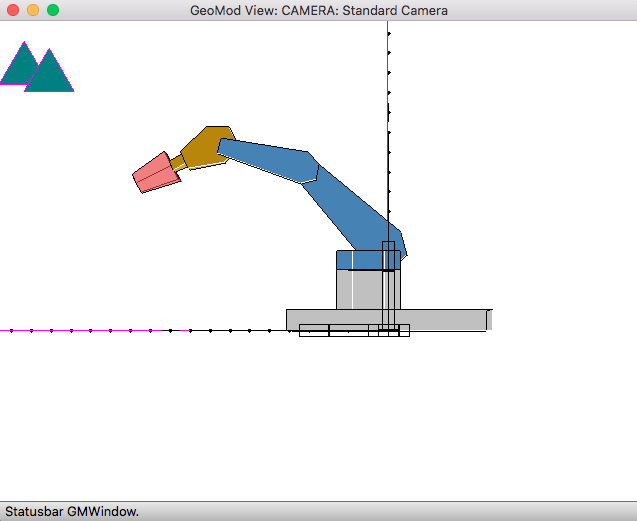
\includegraphics[height=8cm]{images/GeometricModel.png}
    \captionsource{\url{http://mathworld.wolfram.com/images/eps-gif/DualsPlatonicSolids_1000.gif}}
    \caption[Polyhedrons]{Polyhedrons}
    \label{fig:polyhedrons}
\end{figure}



\subsection{Tools and Paths}
GeomEdge og GeomNode


Endring i  bibliotek for håndtering  av  bevegelse  i  bestemt  referanse  -  nevne  basis  o gimplentasjon av en slik funksjon til hver akse.

\subsection{Control System}
Translation, orientation, rotation, position. Cartesian. TGroup. Basis. offset vector.



